\documentclass[12pt]{article}

\usepackage{amsmath}
\usepackage[usenames,dvipsnames,svgnames,table]{xcolor}
\usepackage[colorlinks=true,citecolor=brown]{hyperref}
\usepackage{graphicx}
\usepackage{natbib}
\usepackage{setspace}
%\doublespacing

\begin{document}

%%%%%%%%%
\title{Molecular Clock Dating using MrBayes}
\author{Chi Zhang$^{1,2,*}$}
\maketitle

\noindent{\it
$^1$Department of Bioinformatics and Genetics, Swedish Museum of Natural History, Box 50007, 10405 Stockholm, Sweden; \\
$^2$Department of Biosystems Science and Engineering, Eidgen\"{o}ssische Technische Hochschule Z\"{u}rich, 4058 Basel, Switzerland; \\
$^*$E-mail: zhangchicool@gmail.com
}

%%%%%%%%%
\newpage 
MrBayes is a software for Bayesian phylogenetic inference \citep{Huelsenbeck:2001jt,Ronquist:2003gt}.
Many new features have been implemented since version 3.2 \citep{Ronquist:2012ir}, 
including species tree inference under the multi-species coalescent model (BEST algorithm) \citep{Liu:2007du};
compound Dirichlet priors for branch lengths \citep{Rannala:2012ke,Zhang:2012ke};
divergence time estimation using node dating \citep{Hedges:2004cl,Yang:2006eu,Ho:2009gn} or total-evidence dating \citep{Ronquist:2012ea,Zhang:2016kf} methods under (relaxed) molecular clock \citep{Huelsenbeck:2000ic,Thorne:2002il,Drummond:2006kt,Lepage:2007bq};
marginal model likelihood estimation using stepping-stone sampling \citep{Xie:2011it};
topology convergence diagnostics using the average standard deviation of split frequencies (ASDSF) \citep{Lakner:2008dn};
BEAGLE library \citep{Ayres:2012gf} support and parallel computing using MPI \citep{Altekar:2004jz}; among others.

There are two modern approaches on dating species divergence using molecular data: node dating \citep[e.g.,][]{Yang:2006eu,Drummond:2006kt} and total-evidence dating \citep[e.g.,][]{Ronquist:2012ea,Zhang:2016kf}.
In a Bayesian framework, node dating calibrates one or several internal nodes of the tree, each with a prior distribution derived from the fossil record. 
While total-evidence dating uses the morphological data from the fossil record and morphological and sequence data from extant taxa together to infer the tree and divergence times. The age of each fossil is assigned a prior distribution directly.

Several steps involve in Bayesian dating analysis, importantly including data partitioning, specifying evolutionary model, calibrating internal nodes or fossils, and setting priors for the tree and the molecular clock model.
In this tutorial, I demonstrate the molecular clock dating functionalities in MrBayes 3.2 step by step, while focusing on total-evidence dating, using an example dataset truncated from the Hymenoptera data analyzed in \citet{Ronquist:2012ea,Zhang:2016kf}. 

%%%%%%%%%
\section{Getting Started}

The program MrBayes is available from \url{http://mrbayes.net} (latest version 3.2.7).
After downloading and installing MrBayes by following the manual, we execute the program from terminal (or command prompt) by typing {\tt \color{blue} mb}
(assuming the executable is in the user path and is named {\tt \color{blue} mb} on Mac OSX/Linux or {\tt \color{blue} mb.exe} on Windows).

{\tt \center
                        MrBayes v3.2 \\
               (Bayesian Analysis of Phylogeny)\\
        Distributed under the GNU General Public License\\
MrBayes >
}

The prompt {\tt MrBayes >} at the bottom means that MrBayes is running and ready for your commands.
In the following tutorial, the commands for MrBayes are colored {\color{red} RED}, the commands typing in terminal (or command prompt) are colored {\color{blue} BLUE}.

{\noindent \color{red} (!!)}
Direct copy and paste the commands here may result in improper spacing or line breaking in the program. Please copy the plain-text commands included in the example file.

%%%%%%%%%
\section{Run the analyses}
\subsection{Partition the data}

The full data includes 60 extant and 45 fossil hymenopteran taxa and 8 outgroup taxa. The alignment is divided into 8 partitions \citep{Ronquist:2012ea}.
To make it computationally tractable for this tutorial, the data is truncated to 10 extant taxa (including 1 outgroup and 9 hymenopteran taxa) and 10 fossils.
Only the morphology (200 characters), 16S (100 sites) and EF1$\alpha$ (210 sites) partitions are included, all partially.
% This example data is available from \url{https://sourceforge.net/p/mrbayes/code/HEAD/tree/test/hym.nex}.

Use the {\tt execute} command ({\tt exe} for short) to read in the data named {\tt hym.nex}.

\medskip
{\tt \color{red} \noindent
execute hym.nex
}
\medskip

\noindent The following commands partition the data into four partitions:
the morphology, 16S, 1st and 2nd codon positions of Ef1$\alpha$, and 3rd codon positions of Ef1$\alpha$,
and exclude the incompatible (constant) characters
(these commands are included in the example data and have been executed automatically when reading it in).

\medskip
{\tt \color{red} \noindent
charset MV = 1-200      \\
charset 16S = 201-300   \\
charset Ef1a = 301-510  \\
charset Ef1a12 = 301-510\textbackslash 3 302-510\textbackslash 3 \\
charset Ef1a3 = 303-510\textbackslash 3         \\
partition four = 4: MV, 16S, Ef1a12, Ef1a3      \\
set partition = four    \\
exclude 7 31 61 83 107 121 122 133 182 183 198
}
\medskip

It is much worth mentioning that the build-in help in MrBayes is very informative and explanatory. We can type {\tt \color{red} help} followed by the keyword to retrieve the corresponding help message. For example,

\medskip
{\tt \color{red} \noindent
help charset   \\
help partition \\
help lset
}
\medskip

\subsection{Evolutionary model}

%% substitution model

For the morphology partition, we use the $Mk$ Model \citep{Lewis:2001wu} with variable ascertainment bias (only variable characters scored), equal state frequencies and gamma rate variation across characters.

\medskip
{\tt \color{red} \noindent
lset applyto = (1) coding = variable rates = gamma
}
\medskip

\noindent If instant change is only allowed between adjacent states (e.g., only 0 $\leftrightarrow$ 1 and 1 $\leftrightarrow$ 2), these characters are specified using {\tt ctype ordered}.
The other characters are thus allowed to change instantly from one state to another.

\medskip
{\tt \color{red} \noindent
ctype ordered$\colon$ 20 23 27 30 36 41 42 44 46 48 59 65 75 78 79 89 \\
\indent               99 112 117 134 146 157 159 171 185 191 193 196
}
\medskip

For the molecular partitions, we use the general time-reversible model with gamma rate variation across sites (GTR$+\Gamma$) \citep{Yang:1994vo,Yang:1994wd}.
The widely used invariable sites and gamma ($+$I$+\Gamma$) model is pathological due to strong correlation between the proportion of invariable sites ($p_0$) and the gamma shape parameter ($\alpha$) \citep[e.g.,][]{Zhang:2012ke}, and is avoided.

\medskip
{\tt \color{red} \noindent
lset applyto = (2,3,4) nst = 6 rates = gamma
}
\medskip

The numbers after {\tt applyto} should match the order of partitions defined above.
The default prior for the shape parameter $\alpha$ of gamma($\alpha$, $\beta$) ($\alpha = \beta$, Figure \ref{fig_gamma}) is exponential(1.0), which can be changed using {\tt \color{red} prset shapepr}. We keep the default here.

\begin{figure}[h]
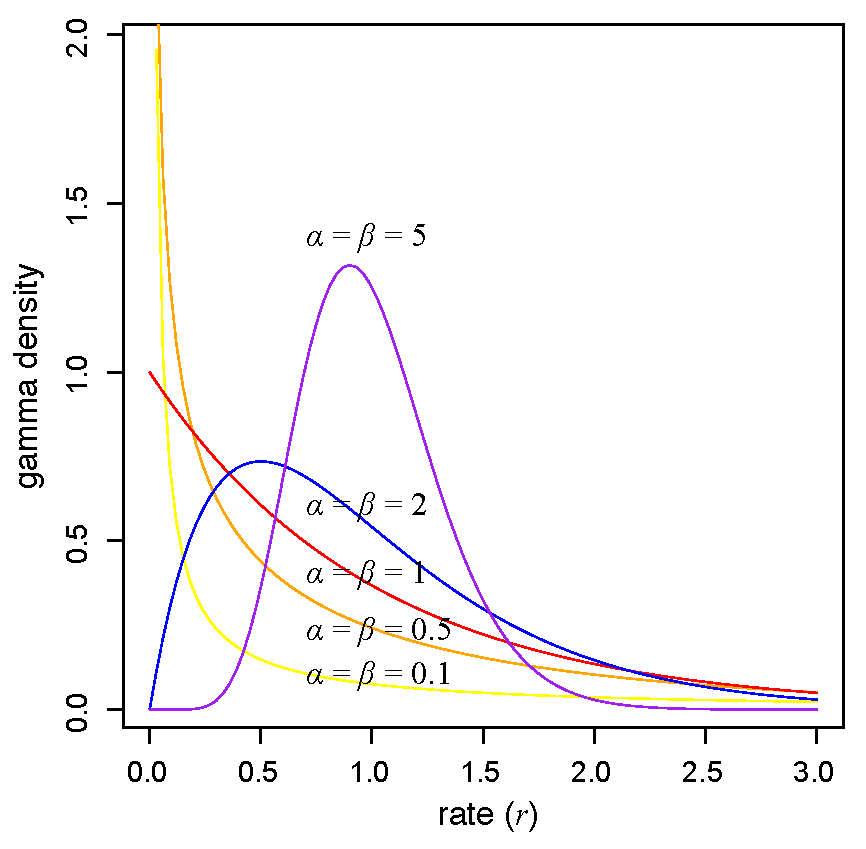
\includegraphics[width=0.7\textwidth]{figures/gamma.pdf}
\caption{Probability density function of the gamma distribution. The shape $\alpha$ and rate $\beta$ are fixed equal so that the mean is 1.0.
The exponential distribution is a special case of gamma when $\alpha = 1$.}
\label{fig_gamma}
\end{figure}

Different partitions are assumed to have independent substitution parameters, thus we unlink them. 

\medskip
{\tt \color{red} \noindent
unlink statefreq = (all) revmat = (all) shape = (all)
}
\medskip

It is reasonable to account for evolutionary rate variation across partitions, so that different partitions can have different substitution rates.

\medskip
{\tt \color{red} \noindent
prset applyto = (all) ratepr = variable
}
\medskip

\noindent The partition-specific rate-multipliers, \{$m_i$\}, have mean equal to 1.0.
Specifically, $\sum_i p_i m_i = 1$, where $p_i$ is the proportion of sites in partition $i$ to the total number of sites.
By default, {\tt ratepr = variable} specifies a uniform Dirichlet prior for \{$p_i m_i$\} (A special case of Dirichlet is uniform on 2 partitions).
Note the difference between partition-specific rate and site-specific rate inside a partition. The sites in partition $i$ have the same partition-specific rate $m_i$, while each site again has a site-specific rate $r_i$ from gamma($\alpha_i$, $\alpha_i$) distribution in the $+\Gamma$ model.

%% relaxed clock model

Molecular data only provide evolutionary distances in units of evolutionary change, such as substitutions per site.
Branch lengths thus are the product of the geological time duration (e.g. in Myr) and the evolutionary rate (e.g. in substitutions per site per Myr).
To estimate times and rates separately, it is necessary to introduce additional model assumptions.

Early studies assumed the evolutionary rate is constant over time (called global clock or strict clock) \citep{Zuckerkandl:1965vq}.
To set a strict clock model with mean rate at 0.001 per site per Myr, we can use a lognormal(-7,0.6) prior for the clock rate, $c$.
The branch length $v_j$ is the geological time duration $t_j$ multiplied by $c$.

\medskip
{\tt \color{red} \noindent
prset clockratepr = lognorm(-7,0.6) \\
prset clockvarpr = strict
}
\medskip

\begin{figure}[h]
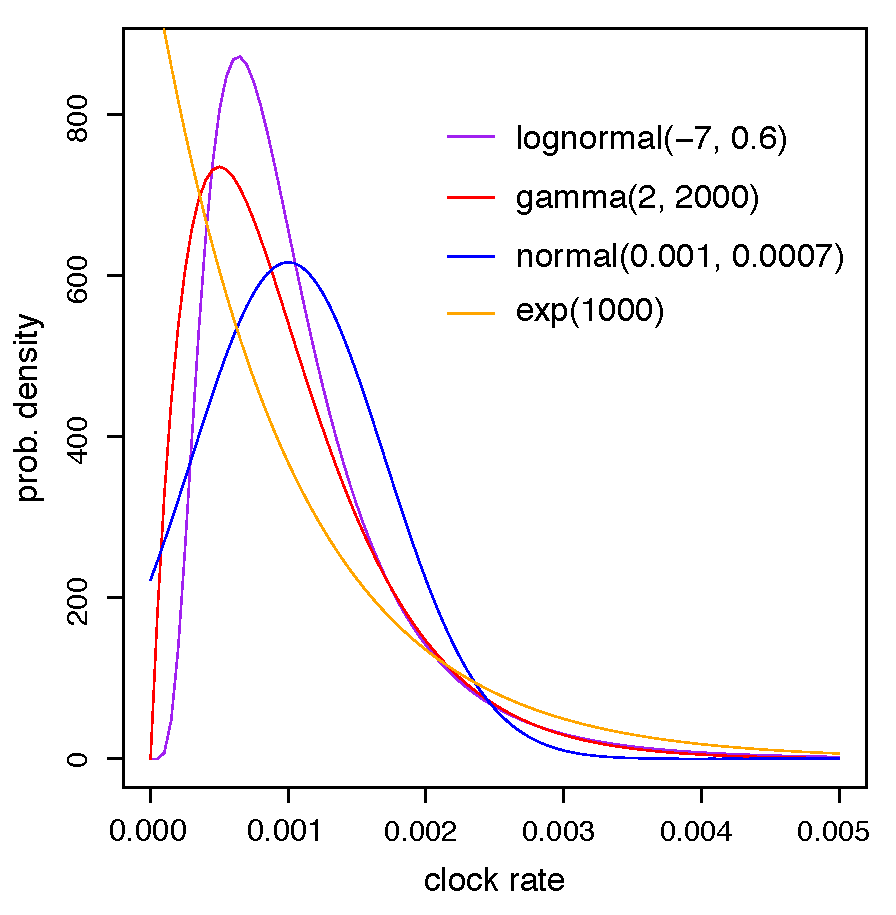
\includegraphics[width=0.7\textwidth]{figures/clockr.pdf}
\caption{Probability density functions of normal, lognormal and gamma distributions, all with mean 0.001 and standard deviation 0.0007. The exponential distribution has mean and standard deviation both equal to 0.001.
}
\label{fig_clockr}
\end{figure}

\noindent There are several options for the clock rate prior, including {\tt fixed}, {\tt normal} (truncated at 0), {\tt lognormal}, and {\tt gamma} (use {\tt \color{red} help prset} for more details).
The probability density functions of the distributions (all with mean 0.001) are shown in Figure \ref{fig_clockr}.
Here I take some space to explain the lognormal distribution, as I think it is confusing.
If $x \sim $ lognormal($\mu$, $\sigma$) then $log(x) \sim $ normal($\mu$, $\sigma$).
The mean of $x$ is $e^{(\mu + \sigma^2/2)}$ and the median of $x$ is $e^{\mu}$.
The variance of $x$ is $(e^{\sigma^2} -1) e^{(2\mu + \sigma^2)}$.
Thus the mean for lognormal(-7, 0.6) is $e^{(-7 + 0.6^2/2)} = 0.001$ and the standard deviation is $\sqrt{(e^{0.6^2} -1) e^{(-2 \times 7 + 0.6^2)}} = 0.0007$.

It is more realistic to assume variable evolutionary rate over time. 
There are three relaxed clock models implemented in MrBayes: compound Poisson process \citep[CPP,][]{Huelsenbeck:2000ic}, autocorrelated lognormal \citep[TK02,][]{Thorne:2002il} and independent gamma rate \citep[IGR,][]{Lepage:2007bq}.
We just focus on the IGR and TK02 model, as the CPP model is not working currently for total-evidence dating (see below). 

\begin{figure}[h]
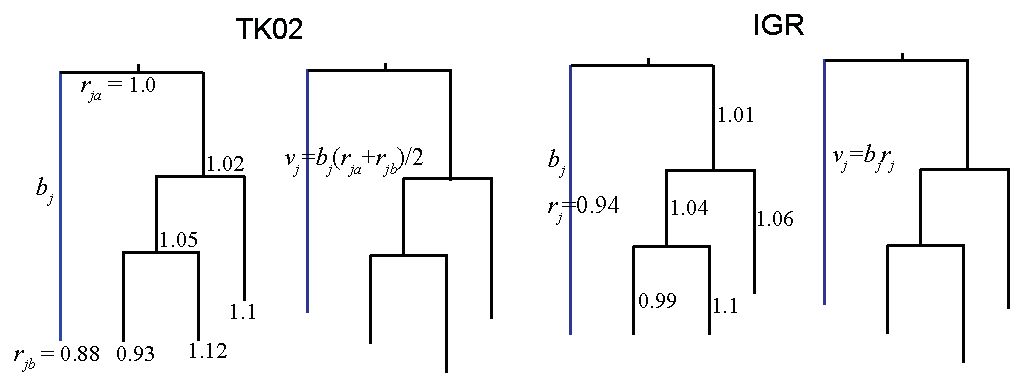
\includegraphics[width=1.0\textwidth]{figures/relaxcl.pdf}
\caption{Illustration of the TK02 and IGR relaxed clock models.
The relaxed clock tree on the right is resulted from the strict clock tree by multiplying its branch lengths with the relaxed clock rates.
}
\label{fig_relaxcl}
\end{figure}

In the TK02 model (Figure \ref{fig_relaxcl}), the (relative) evolutionary rate changes along the branches as Brownian motion on the log scale, starting from 1.0 (0.0 on the log scale) at the root.
The rate at the end of a branch $j$ on the tree is lognormal distributed with mean  (not the log of the mean) equal to the rate at the beginning of the branch
and variance equal to $b_j \sigma^2_{TK}$, where $b_j$ is the product of geological time duration $t_j$ and the base clock rate $c$.
The branch length $v_j$ is then calculated as $b_j$ multiplied by the arithmetic mean of the two rates at both ends.
The TK02 model is specified using

\medskip
{\tt \color{red} \noindent
prset clockvarpr = tk02
}
\medskip

\noindent The prior for $c$ was already set above using {\tt clockratepr}. The prior for $\sigma^2_{TK}$ is specified by 

\medskip
{\tt \color{red} \noindent
prset tk02varpr = exp(1)
}
\medskip

The IGR model assumes that the (relative) rate for branch $j$ is gamma distributed with mean 1.0 and variance $\sigma^2_{IG}/b_j$ (Figure \ref{fig_relaxcl}).
The rates for different branches are independent but not identical.
The branch length $v_j$ is then calculated as $b_j$ multiplied by the branch rate.
In equivalent, $v_j$ is gamma distributed with mean $b_j$ and variance $b_j \sigma^2_{IG}$ \citep[original definition in][]{Lepage:2007bq}. 
The IGR model is specified using

\medskip
{\tt \color{red} \noindent
prset clockvarpr = igr
}
\medskip

\noindent and the prior for $\sigma^2_{IG}$ is specified by 

\medskip
{\tt \color{red} \noindent
prset igrvarpr = exp(10)
}
\medskip

Note that when the branch rates are all fixed to 1.0 for TK02 or IGR, it becomes the strict clock model.
For the likelihood calculation \citep{Felsenstein:1981vk}, the evolutionary distance (number of substitutions per site) for branch $j$, site $k$ in partition $i$ is $d_{jik} = v_{j} m_i r_{ik}$ 
(where $m_i$ is the partition-specific rate, $r_{ik}$ is the site-specific rate).

Before doing total-evidence dating and node dating, we first define the outgroup and fossil group,

\medskip
{\tt \color{red} \noindent
outgroup Raphidioptera  \\
taxset fossils = Asioxyela Nigrimonticola Xyelotoma \\
\indent          Undatoma Dahuratoma Cleistogaster  Ghilarella\\
\indent          Mesorussus Prosyntexis Pseudoxyelocerus
}
\medskip

\noindent and some constraints for later use. Note these constraints are {\it not} enforced until we set {\tt topologypr} explicitly (see below).

\medskip
{\tt \color{red} \noindent
constraint root = 1-.           \\
constraint HymenFossil = 2-.    \\
constraint Hymenoptera = 2-10   \\
constraint Holometabola = 1-10  \\
constraint Tenthredinidae = 3-5 \\
constraint CepSirOruApo = 7-10
}
\medskip

\subsection{Total-evidence dating}

In the following, we incorporate fossil information and assign priors for the
geological times.
This is a typical step in total-evidence dating, where we calibrate the fossils instead of the internal nodes.

\medskip
{\tt \color{red} \noindent
calibrate  \\
\indent Asioxyela = unif(228,242)      \\
\indent Nigrimonticola = unif(152,163) \\
\indent Xyelotoma = unif(152,163)      \\
\indent Undatoma = unif(145,152)       \\
\indent Dahuratoma = fixed(134)        \\
\indent Cleistogaster = unif(168,191)  \\
\indent Ghilarella = unif(113,125)     \\
\indent Mesorussus = unif(94,100)      \\
\indent Prosyntexis = unif(80,86)      \\
\indent Pseudoxyelocerus = fixed(182)  \\
prset nodeagepr = calibrated
}
\medskip

\noindent The last command {\tt nodeagepr} is {\it necessary} to enable the calibrations.
There is more information in {\tt \color{red} help calibrate}.

\begin{figure}[h]
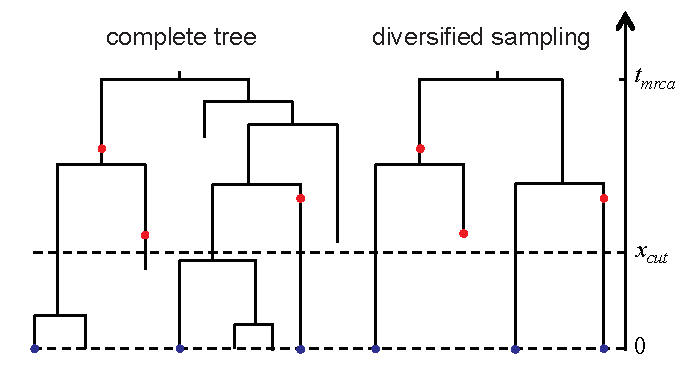
\includegraphics[width=0.9\textwidth]{figures/fbdtree.pdf}
\caption{The fossilized birth-death (FBD) process under diversified sampling.}
\label{fig_fbdtree}
\end{figure}

The speciation, extinction and fossilization process is explicitly modeled using the fossilized birth-death (FBD) process \citep{Stadler:2010fn,Heath:2014hn,Gavryushkina:2014fw,Zhang:2016kf}.
The complete tree is generated from the birth-death process, with speciation rate $\lambda$ and extinction rate $\mu$ (Figure \ref{fig_fbdtree}). 
Two sampling strategies are assumed. For random sampling, the extant taxa are sampled uniformly at random with probability $\rho$, while the fossils are sampled with a constant rate $\psi$ through time.
For diversified sampling \citep{Zhang:2016kf}, exactly one representative taxa per clade descending from time $x_{cut}$ is sampled, resulting a proportion of $\rho$ extant taxa sampled.
The fossils are sampled with a constant rate $\psi$ before $x_{cut}$ and zero after.
The observed FBD tree is resulted when all lineages without a fossil or sampled extant descendant have been pruned.
A fossil can be either tip or ancestor of other taxa (Figure \ref{fig_fbdtree}).

The FBD prior is enabled using

\medskip
{\tt \color{red} \noindent
prset brlenspr = clock:fossilization
}
\medskip

\noindent The sampling proportion $\rho$ is fixed to 0.0001, based on the living number of hymenopteran species at about $10/0.0001=100,000$.

\medskip
{\tt \color{red} \noindent
prset sampleprob = 0.0001
}
\medskip

\noindent The sampling strategy is set to be diversified, as it is arguably suitable for this species-level dataset.

\medskip
{\tt \color{red} \noindent
prset samplestrat = diversity
}
\medskip

\noindent For inference, rather then operating on $\lambda$, $\mu$ and $\psi$, which may range from 0 to infinity, we re-parametrize them as $d = \lambda - \mu$ (net diversification), $e = \mu / \lambda$ (turnover), and $s = \psi/(\mu + \psi)$ (fossil sampling proportion), so that the later two parameters range from 0 to 1.
The default priors for $d$, $e$, and $s$ are:

\medskip
{\tt \color{red} \noindent
prset speciationpr = exp(10)      \\
prset extinctionpr = beta(1,1)    \\
prset fossilizationpr = beta(1,1)
}
\medskip

In order to root the tree properly, we enable the constraint {\tt HymenFossil} defined above.
This forces the Hymenoptera with fossils form a monophyletic group.

\medskip
{\tt \color{red} \noindent
prset topologypr = constraint(HymenFossil)
}
\medskip

The FBD prior is conditioned on the root age of the tree ($t_{mrca}$).
It is important to set it properly.
Here we use an offset exponential distribution with minimal age 300 Ma and mean age 390 Ma.

\medskip
{\tt \color{red} \noindent
prset treeagepr = offsetexp(300,390)
}
\medskip

You may have noticed that various prior distributions for tree age (and for calibration) are available, 
and the way specifying the prior parameters as minimal age and mean age is {\it different} from the parameterization used elsewhere in the program.
This setting is aiming to ease the user and to assure a proper prior is specified.
Several probability densities all with mean 390 and minimal 300 are shown in Figure \ref{fig_treeage}, including the offsetexp(300, 390) and other candidates (offsetlognormal(300, 390, 118), offsetgamma(300, 390, 64), truncatednormal(300, 390, 60)).

\begin{figure}[p]
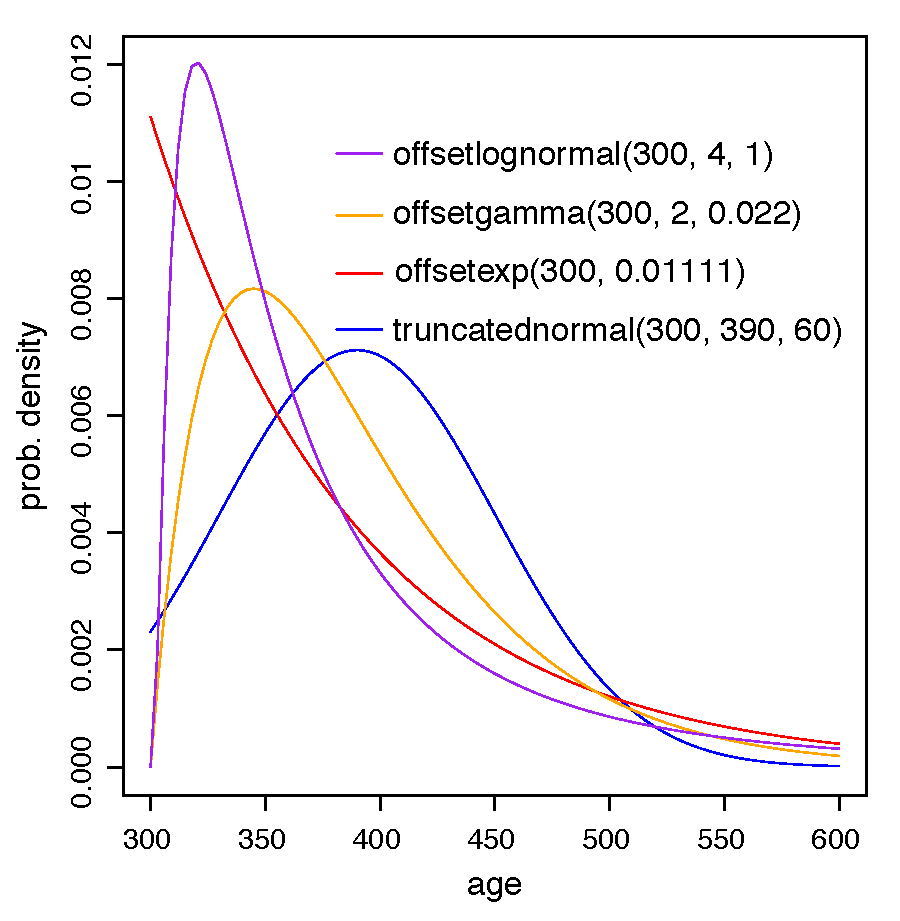
\includegraphics[width=0.7\textwidth]{figures/treeage.pdf}
\caption{Probability density functions of offsetlognormal($m$, $\mu$, $\sigma$), offsetgamma($m$, $\alpha$, $\beta$), offsetexp($m$, $\lambda$), and truncatednormal($m$, $\mu$, $\sigma$).
For offsetlognormal the mean is $m + e^{(\mu + \sigma^2/2)}$ (the median is $m + e^{\mu}$) and the standard deviation is $\sqrt{(e^{\sigma^2} -1) e^{(2\mu + \sigma^2)}}$;
for offsetgamma the mean is $m + \alpha/\beta$ and the standard deviation is $\sqrt{\alpha}/\beta$;
for offsetexp the mean is $m + 1/\lambda$ and the standard deviation is $1/\lambda$;
for truncatednormal the mean is slightly larger then $\mu$ and the standard deviation is slightly smaller then $\sigma$, depending on the left truncation point.
}
\label{fig_treeage}
\end{figure}

Here I mention that there is another tree prior, the uniform prior \\
({\tt clock:uniform}) \citep{Ronquist:2012ea}, that fits in the total-evidence dating framework.
The model assumes that the internal nodes are draw from uniform distributions and the fossils are only tips of the tree (so-called tip dating). 
It is also conditioned on the root age and requires setting {\tt treeagepr}, but there is no speciation-extinction-fossilization-sampling parameter.

All models and priors are set :). To see the current settings, use

\medskip
{\tt \color{red} \noindent
showmodel
}
\medskip

\noindent These messages will also be printed at the beginning of the run.

Now it is time to run the analysis. We first set the Markov chain Monte Carlo (MCMC) \citep{Metropolis:1953vj, Hastings:1970ew} without running it.

\medskip
{\tt \color{red} \noindent
mcmcp nrun = 2 nchain = 4 ngen = 500000 samplefr = 100 \\
mcmcp filename = hym.te  printfr = 1000 diagnfr = 5000
}
\medskip

\noindent This setting uses 2 independent runs and 4 chains (1 cold and 3 heated) per run for 500,000 iterations, and samples every 100 iterations.
The output file names will be hym.te.$*$. The chain states will be printed to screen every 1000 iterations.
The convergence diagnostics (acceptance ratios and average standard deviation of split frequencies (ASDSF)) will be printed every 5000 iterations.
See {\tt \color{red} help mcmc} for other default settings that you may want to change as well.

To run the MCMC, just type

\medskip
{\tt \color{red} \noindent
mcmc
}
\medskip

\noindent then you will see the log likelihoods printed to the screen, with {\tt [ ]} for the cold chain and {\tt ( )} for the hot, and the time left to finish.

\medskip
{\tt \noindent
0 -- [-3530.775] (-3407.296) (-3461.278) (-3476.937) *             \\
\indent   [-3537.572] (-3494.511) (-3460.711) (-3407.261)          \\
1000 -- (-3281.546) [-3286.212] (-3193.371) (-3198.067) *          \\
\indent (-3249.083) (-3208.938) [-3214.627] (-3142.797) -- 0:08:19 \\
$\dots$  \\
\indent Average standard deviation of split frequencies: 0.101638  \\
101000 -- (-2884.632) (-2873.325) (-2869.337) [-2874.607] *        \\
\indent [-2876.804] (-2871.278) (-2872.583) (-2867.121) -- 0:07:22 \\
$\dots$  \\
500000 -- (-2871.038) (-2876.999) (-2866.260) [-2866.105] *        \\
\indent (-2853.373) [-2868.731] (-2881.175) (-2867.806) -- 0:00:00 \\
\indent Average standard deviation of split frequencies: 0.085192  \\
Continue with analysis? (yes/no): no  \\
$\dots$
}
\medskip

\noindent The ASDSF is decreasing slowly toward 0, indicating the tree topologies sampled from different runs are getting similar and converging to the same (stationary) distribution.
We stop the run by typing {\tt no} when prompted.
Then at the end, it will print the chain swap information.

To summarize the results, we use

\medskip
{\tt \color{red} \noindent
sump  \\
sumt
}
\medskip

First we look at the outputs from {\tt sump}.
The likelihood traces for the two runs are mixed together, this is also a good indication of convergence. It also helps us to determine the number of burnin.
By default, 25\% of the samples are discarded. This can be changed by {\tt sump burninfrac = 0.4}, say. 
The traces are followed by a table of the parameter estimates.
Since MCMC is sampling correlated samples, the effective sample size (ESS) is smaller than the actual number of samples (500000/100=5000 in this example).
Ideally ESS should larger than 200 for all parameters to make good estimates.
We do not run longer for this tutorial, but note that we can increase the number of iterations and append to the current samples.

\medskip
{\tt \color{red} \noindent
mcmc ngen=1000000 append=yes
}
\medskip

Then go the the outputs from {\tt sumt}.
It first lists the taxon bipartitions and the corresponding IDs.
The root ID is 0; the extant taxa IDs are 1 to 10; the fossil IDs are 11 to 20.
The following summaries are matched to the bipartition IDs.
The tree is printed at the end.

The consensus tree including all fossils is highly unresolved due to uncertainty in the placement of the fossils.
In order to display the ages clearly, we remove the fossils and redraw an extant taxa tree. The output filename is changed to avoid overwriting the existing ones.

\medskip
{\tt \color{red} \noindent
delete fossils  \\
sumt output = hym.rf
}
\medskip

\subsection{Node dating}

In node dating, we calibrate internal nodes instead of fossils.
The calibration priors are derived from second interpretation of the fossil record.
Thus we remove the fossils, the morphological characters of fossils are not used.

\medskip
{\tt \color{red} \noindent
delete fossils \\
exclude 24 130 168
}
\medskip

Then we calibrate the root, and another two internal nodes.
These three probability densities are shown in Figure \ref{fig_nodecali}.

\medskip
{\tt \color{red} \noindent
calibrate  \\
\indent root = offsetexp(300,390) \\
\indent Tenthredinidae = offsetgamma(100,150,25)   \\
\indent CepSirOruApo = truncatednormal(140,175,25) \\
prset nodeagepr = calibrated
}
\medskip

\noindent Note that the root age calibration here is equivalent to {\tt prset treeagepr \\ = offsetexp(300,390)} (see above), thus either of them is sufficient.

\begin{figure}[h]
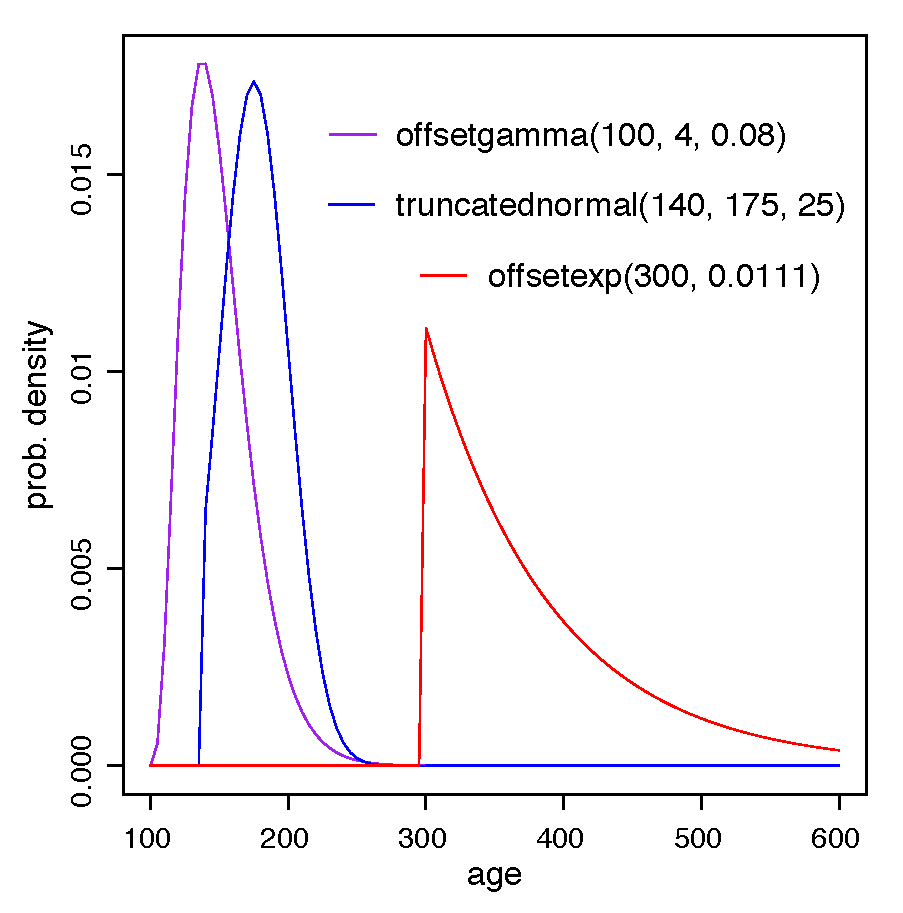
\includegraphics[width=0.7\textwidth]{figures/nodecali.pdf}
\caption{Probability density functions of offsetexp(300, 0.011) (offsetexp(300, 390) in MrBayes), offsetgamma(100, 4, 0.08) (offsetgamma(100, 150, 25) in MrBayes), and truncatednormal(140, 175, 25).
}
\label{fig_nodecali}
\end{figure}

We can still use the FBD prior but fix the fossilization rate to 0 (no fossil sampling).

\medskip
{\tt \color{red} \noindent
prset fossilizationpr = fixed(0)
}
\medskip

\noindent Alternatively, we can use the birth-death prior.

\medskip
{\tt \color{red} \noindent
prset brlenspr = clock:birthdeath
}
\medskip

\noindent Comparing to the FBD prior, the birth-death prior does not assume fossil sampling, thus {\tt fossilizationpr} is irrelevant. 
The priors for the root age, speciation rate, extinction rate, sampling strategy (diversified) and sampling proportion (0.0001) are not changed (see above).

The uniform tree prior ({\tt clock:uniform}) is also applicable, then the speciation-extinction-fossilization-sampling priors are irrelevant.

It is important to force the calibrated node to be monophyletic, and enable the constraints using

\medskip
{\tt \color{red} \noindent
prset topologypr = constraint(Hymenoptera,  \\
\hspace*{5cm} Tenthredinidae,CepSirOruApo)
}
\medskip

\noindent The Hymenoptera constraint helps to root the tree properly.

We change the output filename to avoid overwriting existing ones.
We also need to reset the starting values, as this node dating run is continued after the total-evidence dating run in the same session.

\medskip
{\tt \color{red} \noindent
mcmcp filename = hym.nd startp = reset startt = random
}
\medskip

\noindent The other settings are kept the same as in total-evidence dating above.

\medskip
{\tt \color{red} \noindent
mcmc  \\
sump  \\
sumt
}
\medskip

\subsection{Batch mode}

In practice, instead of typing commands line by line in MrBayes, we usually write the commands in file, either after the data block as in this example, or in separate files.
Each command should end with a semicolon {\tt \color{red} ;}.
Texts in a pair of square brackets {\tt [ ]} is a comment, and is ignored by the program.
Below is an example of commands in a separate file (named {\tt mbcmd.nex}), in the same folder as {\tt hym.nex}.

\medskip
{\tt \noindent
\#NEXUS        \\
Begin mrbayes; \\
\indent [read in data] \\
\indent exe hym.nex; \\
\indent [partition data] \\
\indent \dots  \\
\indent [model and prior] \\
\indent \dots  \\
\indent prset brlenspr = uncons:gammadir(1,1,1,1); \\
\indent \dots  \\
\indent mcmc;  \\
\indent sump;  \\
\indent sumt;  \\
end;
}
\medskip

\noindent To run the analysis, just type

\medskip
{\tt \noindent \color{red} execute mbcmd.nex}
\medskip

\noindent after the {\tt MrBayes >} prompt (MrBayes is running), or

\medskip
{\tt \noindent \color{blue} mb mbcmd.nex}
\medskip

\noindent in terminal (or command prompt. MrBayes is not running).

\subsection{A non-clock analysis}

Before looking at the results, we do a non-clock analysis without assuming molecular clock, to compare the tree with the relaxed clock tree.
The branch lengths are measured in expected substitutions per site.
This is a typical analysis most people do using MrBayes.

We do not use fossils either, and do not constrain the topology so that they are uniformly distributed.
The evolutionary model is kept the same but the setting for clock rate is ignored. 

\medskip
{\tt \color{red} \noindent
delete fossils  \\
prset brlenspr = uncons:gammadir(1,1,1,1) \\
prset topologypr = uniform  \\
mcmcp filename = hym.un \\
mcmc  \\
sump  \\
sumt
}
\medskip

Note the prior for branch lengths is a gamma-Dirichlet($\alpha_T$, $\beta_T$, $\alpha$, $c$) prior \citep{Rannala:2012ke,Zhang:2012ke}.
The prior assigns a gamma($\alpha_T$, $\beta_T$) distribution for the tree length (sum of branch lengths), and a Dirichlet($\alpha$, $c$) prior for the proportion of branch lengths to the tree length.
In the Dirichlet, the parameter for external branches is $\alpha$ and for internal branches is $\alpha c$, so that the prior ratio between internal and external branch is $c$.
In this case, we assign gamma(1, 1) (i.e. exponential(1), cf. Figure \ref{fig_gamma}) for the tree length and uniform Dirichlet for the proportions.

The gamma-Dirichlet (compound Dirichlet) prior was shown to help avoiding overestimation of tree length \citep{Zhang:2012ke} and is now the default prior in MrBayes (after v3.2.3).
It was independent and identically distributed (i.i.d.) exponential(10) for each branch length before.
For this 10 extant taxa example, the prior distributions for the tree length and for each branch length are shown in Figure \ref{fig_gamdir}.
The gamma-Dirichlet prior appears less informative and more flexiable than the i.i.d. exp(10).

\begin{figure}[p]
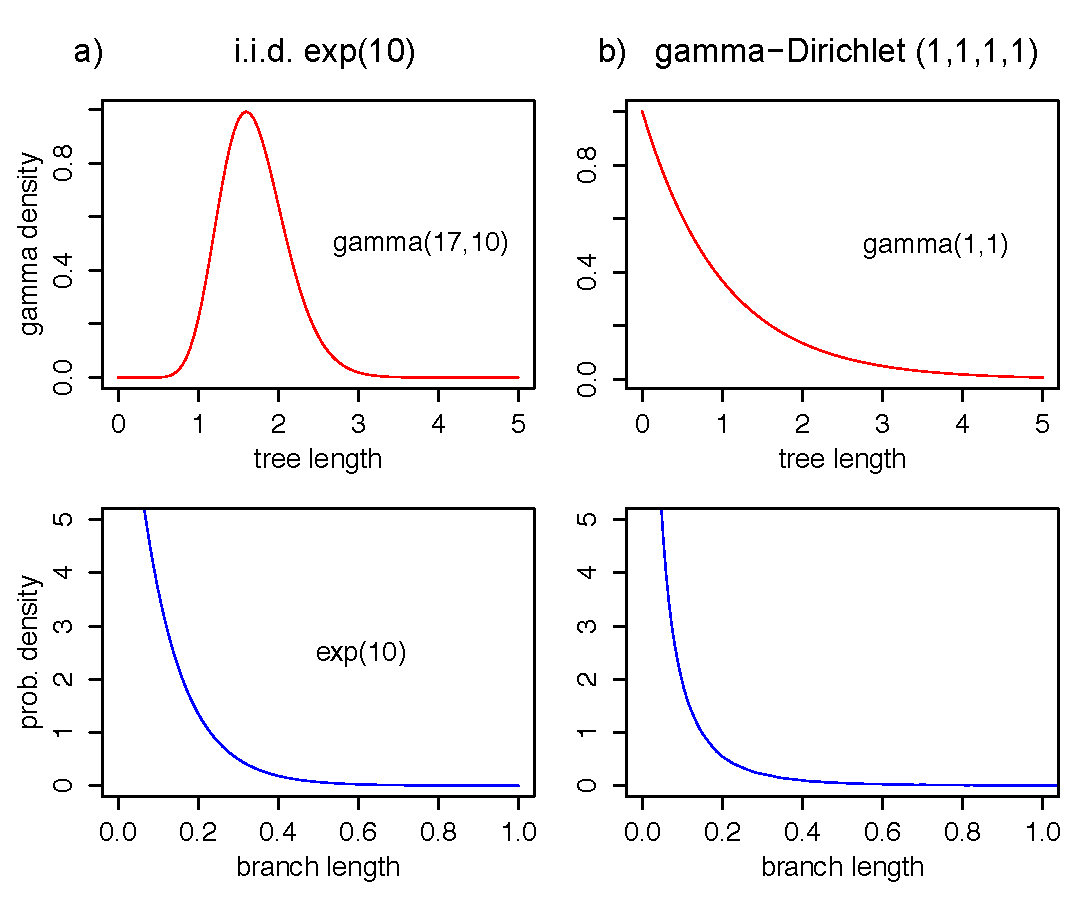
\includegraphics[width=1.0\textwidth]{figures/gamdir.pdf}
\caption{Probability densities for the tree length and for each branch length under a) i.i.d. exponential(10) prior and b) gamma-Dirichlet(1, 1, 1, 1) prior.
The sum of $n$ i.i.d. gamma($\alpha$, $\beta$) is gamma($n \alpha$, $\beta$), and the proportion to the sum is Dirichlet($\alpha$).
Thus the sum of $n = 2 \times 10 - 3 = 17$ i.i.d. exp(10) (gamma(1, 10)) is gamma-Dirichlet(17, 10, 1, 1).
Under gamma-Dirichlet(1, 1, 1, 1), the priors for branch lengths are i.i.d. but not exactly gamma.
}
\label{fig_gamdir}
\end{figure}
\clearpage

%%%%%%%%%
\section{Summarize the results}

The posterior estimates on the screen are also output to files, with names specified using the commands above, each with a particular extension. 
These files can be opened using a plain-text editor. 

The partition rate multipliers $m_i$ are in file {\tt hym.*.pstat}. 
The first and second codon positions ({\tt m\{3\}}) evolve much slower than the third codon position ({\tt m\{4\}}). The morphology ({\tt m\{1\}}) and 16S ({\tt m\{2\}}) partitions evolve at similar rate.

There are many tools to visualize the trees in file {\tt hym.*.con.tre}.
Here I use FigTree \url{http://tree.bio.ed.ac.uk/software/figtree/}.
It is very compatible with the consensus tree format output from MrBayes.
There are various options on the left panel of FigTree to adjust the display.

The clock trees from total-evidence dating and node dating under diversified FBD prior and IGR model are shown in Figure \ref{fig_cltree}.
The ages of root and hymenopteran crown are shown in Table \ref{tab_age}.
These estimates match the corresponding node bars in Figure \ref{fig_cltree}.
The HPD intervals are in file {\tt hym.*.vstat}.
The bipartition ID of {\tt age\{all\}[.]} is in {\tt hym.*.parts}.
The ID for root is 0 which includes all taxa (all {\tt *}), while the ID for Hymenoptera is that excludes the outgroup and fossils ({\tt .*********}). 

\begin{table}[p]
\caption{Ages (Ma) of root and Hymenoptera (median and 95\% HPD) from total-evidence dating and node dating under diversified FBD prior.} 
\label{tab_age} 
\begin{tabular}{lrll}
\hline
    &               & Root                 & Hymenoptera          \\
\hline
IGR &               &                      &                      \\
    &  TE dating    & 305.4 (300.0, 325.0) & 237.6 (206.4, 287.3) \\
    &  Node dating  & 322.4 (300.0, 394.5) & 243.5 (183.4, 310.7) \\
TK02&               &                      &                      \\
    &  TE dating    & 306.2 (300.0, 327.7) & 289.0 (257.6, 314.0) \\
    &  Node dating  & 325.0 (300.0, 404.0) & 236.6 (185.9, 298.6) \\
\hline 
\end{tabular}
\end{table}

Comparing the non-clock tree (Figure \ref{fig_nctree}) with the clock trees (Figure \ref{fig_cltree}), it is obvious that the evolutionary rate is not constant over time.
The Xyela and Onycholyda lineages evolve much slower than the Orussus and Vespidae clade, and there are indeed dramatic rate changes between adjacent branches.
The IGR model is thus presumably more suitable than the autocorrelated TK02 model.

The ages inferred from the total-evidence dating are slightly younger than those from the node dating under the IGR model (Figure \ref{fig_cltree}), with relatively narrower credibility intervals.
The FBD model in the total-evidence dating approach models the fossilization (and sampling) process explicitly and incorporates all available information from fossil record.
In comparison, the node dating approach discards the fossil morphologies and stratigraphic times, but uses second interpretation of the fossil record as node calibration distributions.
Thus the total-evidence dating approach appears more objective and rigorous, and provides an ideal platform for exploring and further improving the models used for Bayesian divergence-time estimation.

\begin{figure}[p]
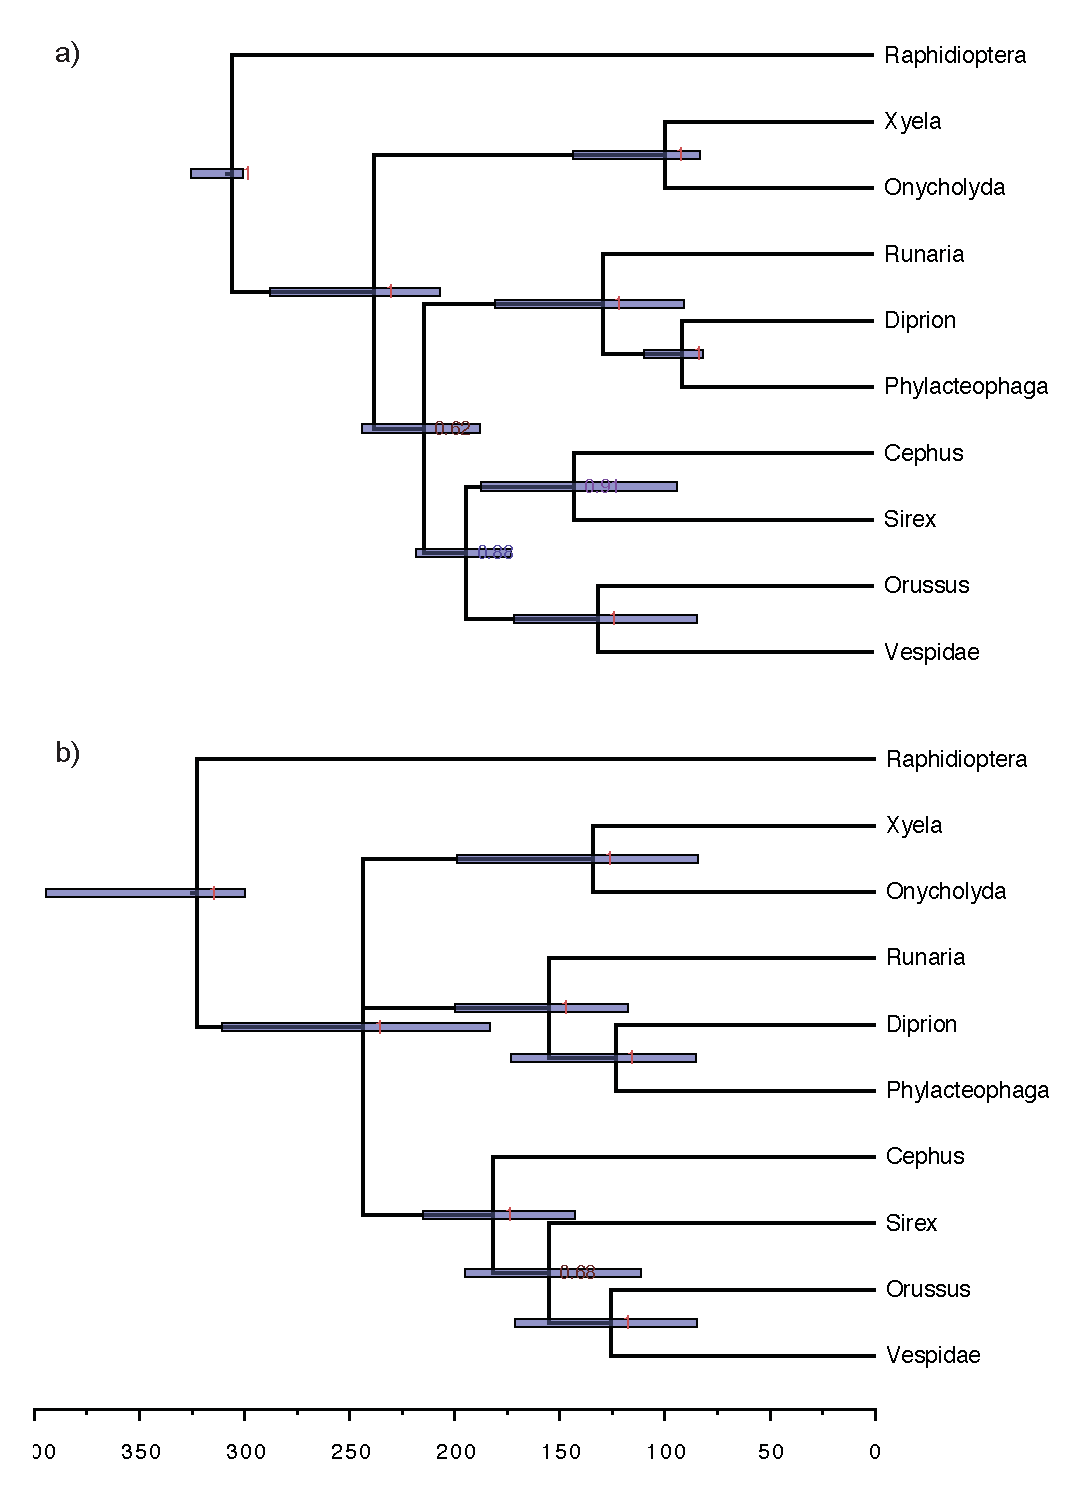
\includegraphics[width=0.9\textwidth]{figures/cltree.pdf}
\caption{Majority-rule consensus trees from a) total-evidence dating and b) node dating, under diversified FBD and IGR model.}
\label{fig_cltree}
\end{figure}

\begin{figure}[p]
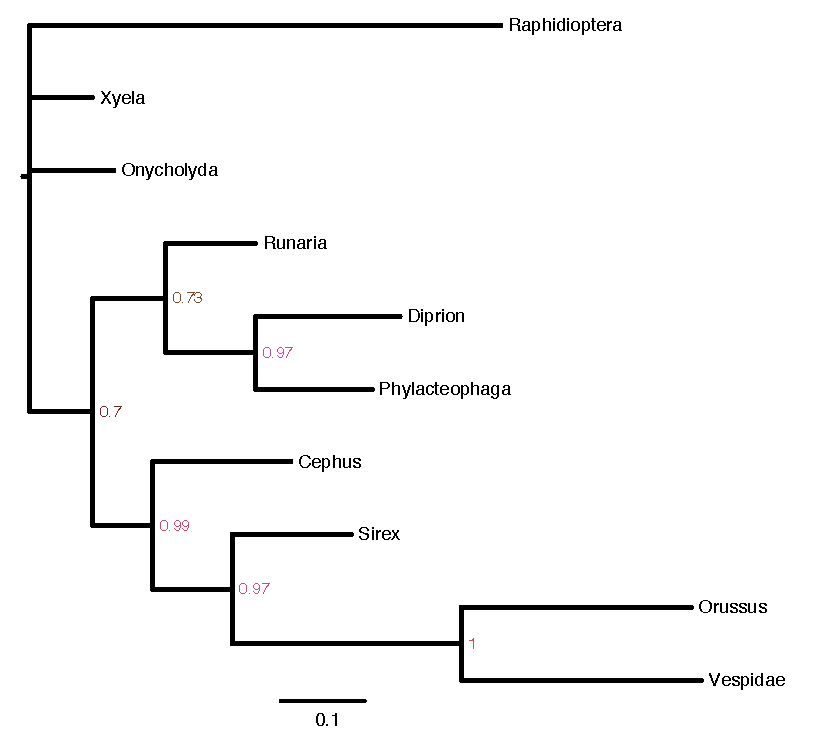
\includegraphics[width=0.8\textwidth]{figures/nctree.pdf}
\caption{Majority-rule consensus tree from non-clock analysis under the gamma-Dirichlet prior.}
\label{fig_nctree}
\end{figure}

Nevertheless, the results from this truncated small dataset are mainly for demonstration of MrBayes' functionalities.
For more results and discussions using the whole data, please see \citet{Ronquist:2012ea,Zhang:2016kf}.

% \section{Model selection using Bayes factor}

\section{Acknowledgements}

I thank Johan Nylander for valuable discussions and for organizing a workshop of MrBayes using this tutorial. 

\bigskip
\noindent \href{http://creativecommons.org/licenses/by/4.0/}{
\includegraphics[scale=0.8]{figures/ccby.pdf}} This tutorial is licensed under a \href{http://creativecommons.org/licenses/by/4.0/}{Creative Commons Attribution 4.0 International License}. 

%%%%%%%%%  REFERENCE    %%%%%%%%%%%%%%%
\newpage
\bibliographystyle{sysbio}
\bibliography{master_refs}

\end{document}
